\chapter{Data Storage - Computer Science Papers Dataset}

\section{The Data Model}
\paragraph{ }The data used for this task was taken from the \texttt{dblp} computer science bibliography dataset\footnote{https://dblp.uni-trier.de/xml/}. This data came in the form of an XML file. The interesting features from this file were extracted and stored as a graph database (using Neo4J) in order to perform the required analysis. The chosen model was quite a simple one and can be seen in Figure \ref{fig::model} where there are two types of nodes (\texttt{Article} and \texttt{Author}) and 1 relationship (\texttt{PUBLISHED}).

\begin{figure}[!b]
	\centering
	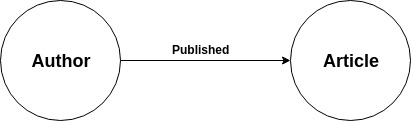
\includegraphics[width=0.6\textwidth]{model}
	\caption[Neo4J Model]{Graph Model Used to Store the \texttt{dblp} Data in Neo4J}
	\label{fig::model}
\end{figure}

\paragraph{ }The \texttt{Author} node simply contains the name of the author. This field was also set as the key since according to the documentation of \texttt{dblp} the name is stored in a way which is guaranteed to be unique. The \texttt{Article} Node, despite its misleading name, stores data on any of the publications listed in the \texttt{bdlp} dataset. This includes articles,articles in proceedings, proceedings, books, articles in collections, PhD thesis, Masters thesis and publications from web sources. These nodes have 2 fields; a key field which contains the unique key identifier assigned to them in the \texttt{dblp} database and the title field containing the name of the publication. Finally, the relationship \texttt{PUBLISHED} contains no fields as it wasn't necessary.

\paragraph{ }In order to import the data into Neo4J, the following steps were done:
\begin{itemize}
	\item Firstly, Neo4J was installed on the local machine. The command \texttt{sudo service neo4j status} was used to check the status of the server and since it was inactive \texttt{sudo service neo4j start} was used to start the server.
	\item The Jupyter Notebook code in `01 - Data Extraction.ipynb' was run to create the data files.
	\item The generated data files were then copied to the Neo4J import directory by running \texttt{sudo cp [file.csv] /var/lib/neo4j/import/[file.csv]} .
	\item Finally, some quotes found in titles of the publications were removed by running \texttt{sudo sed -i 's/\"//g' articles.csv}
\end{itemize}
In particular, in the python file, \texttt{lxml} was first used to extract the required features from the xml file into three csv files (one for each node and one for the relationship). This was slightly tricky to handle due to the size of the xml file and the amount of memory available on the laptop used to run this program. Thus, a generator function was used that would access the xml file element by element rather than storing the whole file in memory. Similarly, the csv files were accessed only when needed in order to ensure that not too much memory we being used. This was a necessary step that traded speed for memory. \texttt{py2neo} was then used to access the database, set the uniqueness constraints on the desired fields in the nodes and load the csv data.

